%\pagenumbering{arabic}%start arabic pagination from 1 

\chapter{Platforma Vert.x}

Dnešním trendem internetu jsou real-time kolaborativní aplikace, které drasticky změnily potřeby programátorů, na jednotlivé nástroje. Programátor tak má možnost zvolit si z velké řádky nástrojů mezi než patří například Node.js, Akka či ruby EventMachine. Problémem těchto jinak časem a komunitou prověřených platforem může být fakt, že jsou úzce spjaté s konkretním programovacím jazykem či velmi náročná integrace do již stávájící aplikace.

Vert.x je projekt vycházející z Node.js, který jako první framework, pokořil v roce 2010 C10K\footnote{C10K problém řeší otázku: „Jak je možné obsloužit deset tisíc klientů za pomocí jednoho serveru, a to s co možná nejnižším zatížením serveru} problém. Platforma Vert.x má velice podobné API\footnote{Application Programming Interface} jako Node.js. Obě platformy poskytují kompletně asynchronní API. Jak již název napovídá Node.js je napsán v JavaScriptu, zatím co Vert.x je implementován v Javě. Vert.x ale nění pouhá reimplementace Node.js do jazyka Java. Platforma má svou vlastní unikátní filozofii, která je diametrálně odlišná od Node.js.

%Problém těchto jinak časem a komunitou ověřených platforem je fakt. Obě zmíněné platformy jsou napsány v dynamicky kompilovaném jazyku, což pro jádro stabilní aplikace přináší povinnost psát jak testy integrační, které testují funkčnost celého systému, tak i unit testy. 
%I když bude aplikace z větší části pokrytá testy, mohou se objevit problémy v podobě nečekaných pádů za běhu aplikace. To může být způsobeno například voláním neexistující metody či přiřazení proměnné do jiného typu než je ona sama. Toto bylo jedním z důvodů pro implementaci nového řešení v jazyce Java. Tento jazyk přináší platformě velkou stabilitu, rozšiřitelnost a zázemí v podobě tisícovek stabilních knihoven. Vert.x může být použit jako plnohodnotné řešení pro celou aplikaci nebo nasazen jako dílčí část architektury jiného řešení.

\section{Historie}

Začátek vývoje projektu Vert.x je datován do roku 2011. Tedy rok poté co spatřil světlo světa framework Node.js a za pouhý rok si vydobyl své místo u komunity, která si jej velmi oblíbila. Pravděpodobně největší motivací pro vývoj nové platformy podobné Node.js byla právě oblíbenost Node.js. 

Hlavním autorem platformy byl a je Tim Fox, který v době začátku vývoje platformy pracoval ve společnosti VMWare. Tato společnost si vzápětí nárokovala všechny zásluhy Tima Foxe na Vert.x platformu. Právníci společnosti vydaly výzvu, ve které požadovali mimo jiné doménu, veškerý zdrojový kód a účet Tima Foxe na Githubu. Z toho důvodu Tim Fox odešel od společnosti v roce 2012. V témže roce projevila o platformu zájem firma RedHat, která nabídla Timovi pracovní místo, absolutně volnou ruku ve vývoji a vedení projektu\citep{whoControlVertx}. 

Po několika debatách jak s představiteli společnosti RedHat tak i komunitou došel Tim Fox k názoru, že nejlepší pro budoucí zdravý rozvoj platformy bude přesunutí celé platformy pod nadaci Eclipse Foundation, k čemuž došlo na konci roku 2013. V dnešní době se platforma těší velkému vývoji, který čítá desítky  pravidelných přispěvatelů mezi něž patří mimo Tima například také Norman Maurer, který patří mezi přední inženýry vyvíjející framework Netty.io, který zodpovídá za integraci Netty frameworku do Vert.x platformy. 

Na tomto místě by bylo vhodné uvést, že platforma Vert.x letos vyhrála prestižní cenu "Most Innovative Java Technology" v soutěži JAX Innovation awards\citep{JAX}.

\section{Architektura}

Na obrázku \ref{fig:vertxArchitectureDiagram} jsou znázorněny dvě nezávislé Vert.x instance, které spolu komunikují pomocí zpráv. V levé části je blíže zobrazena jedna Vert.x instance, která bude blíže rozebrána v následujících kapitolách.

\begin{figure}
\begin{centering}
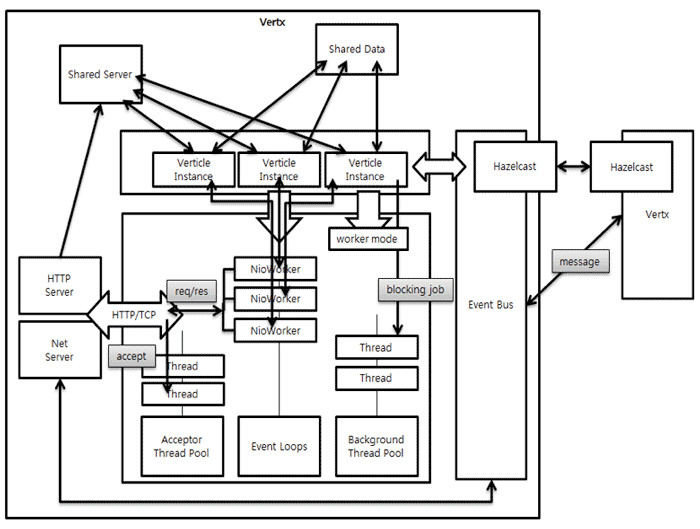
\includegraphics[width	=1\textwidth]{obrazky/vertx-architecture-diagram}
\par\end{centering}
\caption{Architektura Vert.x \emph{Jaehong Kim} \label{fig:vertxArchitectureDiagram}}
\end{figure}

\subsection{Jádro}

Velikost samotného jádra aplikace nepřekračuje 10Mb kódu v jazyce java. V současné verzi je jádro platformy koherentní, dobře čitelné a poskytuje málé, ale za to stabilní API. Jak je popsáno v kapitole \ref{sub:API}, Vert.x se nesnaží umět vše, ale specializuje se na určitou činnost. 

Lze jej následně rozšířit o novou funkčnost dokompilovaním balíčků, které lze naleznout v oficiálním repositáři. Pravděpodobnou inspirací byl již zmíněný Node.js respektive NPM\footnote{Node package manager} u kterého se takováto forma vývoje velice oblíbila. Od doby vzniku této platformy vzniklo nespočet rozšíření, které udělaly z Node.js silný násroj pro rychlý vývoj webových aplikací. 
Klíčové jsou aspekty jako událostmi řízené programování a neblokující asynchronní model.

\subsubsection{Asynchronní model}

Událostmi řízené programování je podle Tomáše Pitnera\cite{javaProgramovani} základním principem tvorby aplikací s GUI(Graphical user interface). Netýká se však pouze GUI, je to obecnější pojem označující typ asynchronního programování, kdy je: tok programu řízen událostmi na které navěšuje tzv. event handlery\footnote{obslužná rutina události}.

Události nastávají obvykle určitou uživatelskou akcí: klik či pohyb myši, stisk tlačítka
událostmi řízené aplikace musí být většinou programovány jako vícevláknové (i když spouštění vláken obvykle explicitně programovat nemusíme)
Asynchronní někdy také paralelní model je přímo závislý na způsobu implementace samotným programovacím jazykem. Základním pojmem je zde proces, který je vnímán jako jedna instance programu, který je plánován pro nezávislé vykonávání. Naproti tomu Vlákno\footnote{Označuje v informatice odlehčený proces, pomocí něhož se snižuje režie operačního systému při změně kontextu, které je nutné pro zajištění multitaskingu} je posloupnost po sobě jdoucích událostí. V dřívější době nebylo potřeba rozlišovat proces a vlákno, protože proces se dále v aplikaci nedělil. Vytvoření vlákna je poměrně drahá a pomalá operace. Což se často obchází vytvořením zásoby uspaných vláken dopředu s nějakým managementem, co vlákna přidává a ubírá dle potřeby. Základním principem Vert.x a jemu podobných frameworků je jedno hlavní vlákno, obvykle pro každý procesor jedno. Takovéto vlákno si pak samo řídí vytváření a přidělování vláken.

Tento model bývá často kritizován, že nutí programátory psát špatně udržovatelný kód, především pak v situacích, kdy je potřeba koordinovat výsledky mezi více handlery. Pro tyhle situace ovšem vznikla řada nástrojů, které se liší podle použitého jazyka.

%respektive Node.js je tedy jedno hlavní vlákno, které si dle potřeby vytváří vlákna další a řídí tak . V jedné aplikace tedy může běžet několik vláken. Vlákno je zde bráno jako základní plánovací jednotka pro běh na procesoru. 
Existují dva druhy asynchronního modelu (multitaskingu):
multiprocesorový: o běh, tvorbu a režii vláken se stará operační systém
multivláknový: o běh, tvorbu a režii vláken se stará aplikace a předává je operačnímu systému
Podle Lažanského\cite{vlaknaCvut} je sdílení paměti důsledkem nižší režie při přepínání (přepnutí vláken je výrazně rychlejší), obdobně i vytváření a rušení vlákna a samozřejmě i úspora paměti.
Jak již bylo zmíněno jádro Vert.x je implementováno v jazyce Java a pro Vert.x je tedy důležité, jak moc je dobrá implementace paralélního modelu v jazyce JAVA. Zde se dostáváme k jedinému požadavku pro běh Vert.x instancí a to je přítomnost Java development Kitu ve verzi 1.7 a novější. Tato verze přinesla nespočet vylepšení, pro jejichž výpis zde není místo. Došlo také na přepsání či úpravy v několika zásadních třídách z balíčku java.util.concurrent, což je třída zabývající se prací s multitaskingem a konkurencí.
\begin{description}
\item[ExecutorService]{z balíčku java.util.concurrent}
\item[CyclicBarrier\footnote{Synchronizační bariéra. Využitelná pro konstantní skupinu vláken, které mají přistupovat ke stejné proměnné. Třída zajištuje, že na sebe vlákna musí čekat při přístupu k proměnným. (Cyklická, protože jakmile se uvolní první vlákno jede to samé od znova)}]{z balíčku java.util.concurrent}
\item[CountDownLatch]{z balíčku java.util.concurrent}
\item[File]{z balíčku java.nio}
\item[Vylepšený ClassLoader\footnote{objekt zajištující načítání tříd}]{lepší odolnost vůči deadlockům\footnote{ je odborný výraz pro situaci, kdy úspěšné dokončení první akce je podmíněno předchozím dokončením druhé akce, přičemž druhá akce může být dokončena až po dokončení první akce.}}
\end{description}
\emph{Více o java.concurrent\cite{javaChangelog}}

Ed Gardoh v roce 2011 ve svém jednoduchém testu\cite{serialTest} prověřil práci s paralelizací úkonů. Z jeho testů vyplývá, že Java 1.7 je až o 40\% rychlejší při práci s vlákny díky nové metodě Fork/Join\cite{forkJoin}.

\subsection{Multi-reactor pattern}

Základ jádra je postaven na tzv. Multi-reactor pattern\cite{eventLoops}, který vychází z Reactor patternu\cite{reactorPattern}, ten lze charakterizovat několika body:

\begin{itemize}
\item{aplikace je řízena událostmi}
\item{na události se registrují handlery}
\item{vlákno zpracovává události a spouští registrované handlery}
\item{toto vlákno nesmí být blokováno\footnote{pokud dojde k zablokování hlavního vlákna dojde k zablokování celé aplikace např.\emph{Thread.sleep(), a další z java.util.concurrent }}}
\end{itemize}

Multi-reactor pattern\cite{eventLoops} se od Reactor patternu liší pouze tím, že může mít více hlavních vláken. Tím přináší Vert.x možnost pohodlně škálovat instance na více procesorových jader. Hlavnímu vláknu, se ve Vert.x komunitě říká \emph{Event Loop}. V komunitách Nginx nebo Node.js se ovšem setkáme spíše s pojmem \emph{Run Loop}. Nevýhoda tohoto modelu je, že nikdy nesmí dojít k blokování hlavního vlákna a také fakt, že platforma Node.js poskytovala jenom jedno vlákno, které šlo škálovat na jednotlivé procesory. Jak je vidět z obrázku \vref{fig:instance} Vert.x platforma poskytuje více hlavních vláken, zpravidla však jedno hlavní vlákno na jeden procesor. Toho lze snadno docílit pomocí \emph{Runtime.getRuntime().availableProcessors()} o kterém se dozvíte více v kapitole \ref{sub:Scaling}. Na obrázku \vref{fig:instance4} pak lze vidět situaci čtyř hlavních vláken na čtyři procesorové jádra.

Příklady blokujících volání:
\begin{itemize}
\item{tradiční API (JDBC, externí systémy)}
\item{dlouhotrvající operace (generování apod.)}
\end{itemize}

\subsubsection{Hybridní model vláken}\label{sub:hybrid}

Platforma Vert.x přišla s inovací v oblasti hlavních vláken a to takovou, že k hlavním \emph{Event loops} přidala další sadu vláken \emph{Background thread pool}, které jsou vyčleněny z hlavní architektury a poskytující samostatnou kapitolu pro škálování aplikace. To lze ostatně vidět na obrázku \vref{fig:vertxArchitectureDiagram}. Díky tomu, lze psát specializované moduly nebo verticle tzv. \emph{workery} pro blokující volání či dlouhotrvající operace aniž by nějak omezovaly běh celé aplikace. Více o \emph{workerech} v kapitole \ref{sub:moduly}.

\subsection{Terminologie}

Vert.x definuje svou vlastní terminologii, která je specifická jen pro tuhle platformu. Před dalším výkladem je tak nutné porozumět jednotlivým pojmům, které budou vysvětleny v následujících podkapitolách.

\subsubsection{Verticle}

Základní jednotka vývoje a nasazení. verticle si lze představit jako kus kódu v jazyce Java pak jako třídu s hlavní metodou. verticle je tak nejmenší funkční jednotkou Vert.x. verticle lze spouštět samostatně přímo z příkazové řádky podobně jako skript. Každý verticle běží ve vlastním vlákně z čehož plynou výhody, ale také nevýhody. Díky tomu, že každý verticle běží ve vlastním vlákně odpadá nutnost zámků nad proměnnýma a nejrůznější synchronizace vláken či deadlocky se tak stávájí minulostí. Vzhledem k tomu, že každý verticle má svůj vlastní classloader nemůže tak sdílet statické metody ani hodnoty proměnných s ostatníma. Sdílet data je tak možné pouze dvěma způsoby.
\begin{itemize}
\item{pomocí Message Queue\cite{mq} dále jen MQ}
\item{SharedData object a SharedSet \emph{vertx.sharedData()}}
\end{itemize}
Objekty v SharedData musí být immutable\footnote{jakmile jednou takovýto objekt vznikne nejde dále měnit jeho proměnné}. V dnešní době je řada MQ frameworků přes které lze vést komunikaci u platformy Vert.x však není potřeba externí služba, protože má vlastní Event Bus o kterém pojednává kapitola \ref{sub:eventBus}. Na obrázku \ref{fig:instance} je vidět jeden verticle v kontextu jedné Vert.x instance. Následuje sumarizace vlastností verticle.

\begin{figure}
\begin{centering}
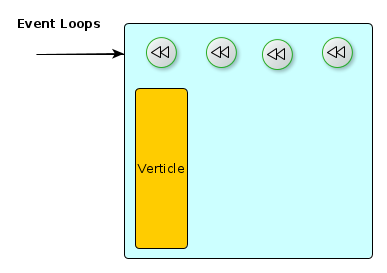
\includegraphics[scale=0.5]{obrazky/instance}
\par\end{centering}
\caption{Vert.x instance \label{fig:instance}}
\end{figure}

\begin{itemize}
\item nejmenší spustitelná jednotka
\item třída / skript
\item vykonává neblokující operace
\item běží vždy v jednom vlákně
\item přímý přístup k API, registrace handlerů, nasazení dalších verticlů
\end{itemize}

\subsubsection{Worker verticle}

V standardním verticlu by nemělo nikdy dojít k blokování hlavního vlákna. V dnešní době se bez klasického synchronního volání pravděpodobně neobejdeme, protože většina knihoven a modulů je napsána jako blokující kód. Z toho důvodu je v platformě Vert.x možnost označit verticle jako workera. Tím dojde k vyčlenění verticle z asociace na hlavní vlákna a takovému vláknu pak bude přiděleno vlákno z Background thread poolu. Uvnitř takového to verticle lze pak vykonávat blokující volání bez blokování celé aplikace. To se v praxi ukázalo jako velice užitečná věc. Bohužel tímto ztrácíme efektivní možnost škálování pro velký počet konkurenčních vláken.

\subsubsection{Vert.x instance}

Každý verticle běží uvnitř Vert.x instance \vref{fig:instance} a každá instance běží ve vlastní JVM instanci. V jedné Vert.x instanci může najednou běžet nespočet Vertclů. Všechny verticle můžou běžet souběžně na jednom serveru. Na jedno serveru může současně běžet mnoho Vert.x instancí v případě clusterování i na více serverech. verticle spolu pak komunikuji pomocí distribuovaného EventBusu.

\begin{figure}
\begin{centering}
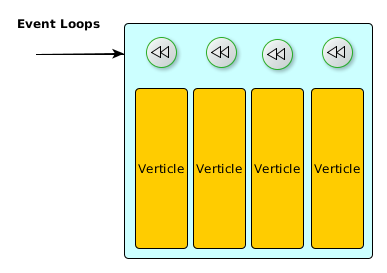
\includegraphics[scale=0.5]{obrazky/instance4}
\par\end{centering}
\caption{Vert.x instance \emph{vertx run HelloWord -instances 4} \label{fig:instance4}}
\end{figure}

\subsubsection{Moduly}\label{sub:moduly}

Moduly poskytují možnost zapouzdření a znovupoužitelnost funkcionality. V praxi se mohou moduly skládat z více modulů či verticlů ve více programovacích jazycích. Modly mohou být uloženy v centrálním repozitáři\footnote{http://modulereg.vertx.io/} nebo může být využit jakýkoliv jiný repozitář. Repozitáře v kterých hledá Vert.x při startu instance dostupné moduly lze definovat v hlavní konfiguraci Vert.x. Každý modul musí mít svůj deskriptor ve formátu JSON\footnote{je odlehčený formát pro výměnu dat}. Jak může vypadat deskriptor je více popsáno v kapitole \ref{sec:praktickyModuly}.

Výhody plynoucí z použití modulů:
\begin{itemize}
\item{classpath\footnote{říká JVM, kde má hledat třídy a balíčky} je zapouzdřený a díky tomu lze moduly pouštět mnohem snáze}
\item{všechny závislosti jsou zapouzdřeny v jediném souboru ve formátu ZIP}
\item{moduly mohou být umístěny v repozitářích}
\item{Vert.x dokáže automaticky stahovat moduly, pokud je nenalezne v lokální instalaci}
\end{itemize}

Typy modulů lze rozdělit do dvou základních skupin, které lze dál rozdělit podle typu určení modulu.

\begin{description}
\item[spustitelné]{mají definovanou hlavní verticle v deskriptoru, takovéto moduly je pak možné spustit jako samostatné jednotky pomocí parametru \emph{runmod} nebo programově \emph{deployModule} }
\item[nespustitelné]{modul nemá specifikovaný hlavní verticle a lze jej použít v jiném modulu použitím metody \emph{includes}}
\end{description}

\subsection{Event Bus}\label{sub:eventBus}

Nervový systém celého Vert.x, jehož název lze volně přeložit jako sběrnice událostí. Cílem EventBusu je zpozdředkování komunikace mezi jednotlivými komponentami a vlákny aplikace. Podobně jako při použití externí MQ. Díky faktu, že komponenta Event Bus je implementována přímo v jádru platformy odpadá nutnost používat další knihovny pro práci s MQ a v neposlední řadě také režijní náklady či výpočetní výkon. Jak je vidět na obrázku , komponenta Event Bus je distribuovaná přes všechny instance v clusteru. Obrovskou výhodou oproti externí MQ je fakt, že lze takovouto komunikaci snadno přemostit ke klientovi na straně webového prohlížeče což je detailněji popsáno v kapitole \ref{sec:realTimeCommunication}.

\begin{figure}
\begin{centering}
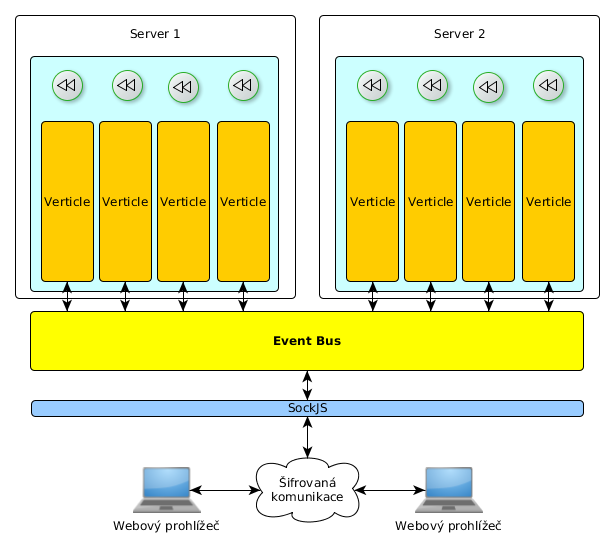
\includegraphics[scale=0.5]{obrazky/2instance4_eventbus}
\par\end{centering}
\caption{Event Bus distribuovaný mezi dva servery}
\label{fig:2instance4_eventbus}
\end{figure}

Základní typy komunikace:
\begin{itemize}
\item{Point to Point}
\item{Publish/Subscribe}
\end{itemize}

typy zpráv:
\begin{itemize}
\item{String}
\item{primitivní typy (int, long, short, float double, ..)}
\item{org.vertx.java.core.json.JsonObject}
\item{org.vertx.java.core.buffer.Buffer}
\end{itemize}

Toto je výčet pouze základních typů zpráv, které Vert.x podporuje v jádře. Není ale vůbec problém výčet stávájících typů rozšířit implementací vlastního modulu. Například modul bson.vertx.eventbus\footnote{https://github.com/pmlopes/mod-bson-io} rozšíří EventBus o možnost používat mnohem komplexnější typy zpráv jejichž výčet se nachází níže.

\begin{itemize}
\item{java.util.UUID}
\item{java.util.List}
\item{java.util.Map}
\item{java.util.Date}
\item{java.util.regex.Pattern}
\item{java.sql.Timestamp}
\end{itemize}

Mezi doporučené se ovšem řadí JSON, protože je jednoduše serializovatelný mezi jednotlivými programovacími jazyky.

\subsubsection{Hazelcast}

Jednou z nejdůležitějších architektonických součástí Vert.x je knihovna Hazelcast, kterou tvoří jenom neuvěřitelných 2,6MB kódu v jazyce Java. Hlavní výhody In-memory data grid\cite{inMemoryDataGrid} lze podle Ki Sun Song sumarizovat:
\begin{itemize}
\item{Data jsou distribuovaná a uložená na více serverech ve více geografických lokacích}
\item{Datový model je většinou objektově orientovaný a ne-relační}
\item{Každý server pracuje v aktivním režimu}
\item{Dle potřeby lze přidávat a odebírat servery}
\end{itemize}

Hazelcast lze využít v několika rolích:
\begin{itemize}
\item{NoSQL databáze v paměti}
\item{Cache\footnote{specializovaný typ paměti pro krátkodobé ukládání}}
\item{Data grid}
\item{Zasílání zpráv}
\item{Aplikační škálování}
\item{Clustrování aplikací}
\end{itemize}

Hazelcast je tedy typ distribuovaného úložiště, které běží jako vestavěný systém a lze díky němu distribuovat celou aplikaci do více geografických lokací nebo zasílat zprávy mezi jednotlivými komponentami. Vert.x API využívá Hazelcast API a odstiňuje tak programátora od poměrně nízko úrovňové API Hazelcastu.Když je Vert.x spuštěn, Hazelcast je spuštěn v módu vestavěného systému. Odpadá tak režie další služby. Jako nejčastější příklad užití samotného Hazelcastu bývá uváděno ukládání uživatelské session\cite{session}. Hazelcast tedy usnadní práci v situaci, kdy budeme potřebovat uložit uživatelskou session například pro eshop. Mohli bychom využít externí RDBMS tedy databázový server, který by obstarával komunikaci s kleinty a udržoval integritu dat díky, kterému by jsme dosáhli stejného výsledku. S využitím knihovny Hazelcast ovšem odpadá nezbytná režie a monitoring, nemluvě o serverových prostředcích.

\section{API}\label{sub:API}

Vert.x poskytuje malou sadu metod, kterou lze volat na přímo z jednotlivých verticlů.
Funkcionalitu platformy lze jednoduše rozšířit pomocí modulů, které po zveřejnění do centrálního repozitáře může využívat kdokoliv a pomáhá tak znovu použitelnosti kódu. Samotné jádro Vert.x je tak velice malé a kompaktní. Vert.x API je rozděleno na \emph{Základní API} a \emph{Kontainer API}.

\subsection{Základní API}\label{sub:coreAPI}

Základní API, které Vert.x poskytuje programátorovi je poněkud strohé a obdobné jako u frameworku Node.js. Platforma tak poskytuje stabilní základ, který se v praxi neobejde bez modulů o kterých pojednává kapitola \ref{sub:moduly}.

\begin{itemize}
\item{TCP/SSL server/klient}
\item{HTTP/HTTPS server/klient}
\item{Websockets server/klient, SockJS}
\item{Distribuovaný Event Bus}
\item{Časovače}
\item{Práce s buffery}
\item{Přístup k souborovému systému}
\item{Přístup ke konfiguraci}
\end{itemize}

\subsection{Kontainer API}

Díky této části API může programátor řídit spouštění a vypínání nových modulů a verticlů za běhu aplikace. V praxi jsme tak schopní škálovat aplikaci za běhu či měnit funkcionalitu celé aplikace aniž by to někdo mohl zaregistrovat. Tuto API můžeme také volat přímo z příkazové řádky dále jen CLI\footnote{Command Line Interface}.

\begin{itemize}
\item{Nasazení a zrušení nasazení verticlů}
\item{Nasazení a zrušení nasazení Modulů}
\item{Získání konfigurace jednotlivých verticlů}
\item{Logování}
\end{itemize}

\subsection{Polyglot}

Polyglot je označován člověk, který ovládá více jazyků. V terminologii Vert.x to znamená, že API je dostupná ve více programovacích jazycích. Což v praxi znamená, že si programátor může sám zvolit v jakém jazyce bude implementovat svůj kód. Díky faktu, že spolu všechny verticly komunikují skrze zprávy je tak možné mít část aplikace napsanou například v jazyce Java a druhou část v jazyce Python apod. Tento fakt hodně napomáhá celé platformě nalákat nové programátory, protože ne každý na světě umí programovací jazyk Java. Výčet podporovaných jazyků ve verzi 2.0. Do verze 3.0 se pak chystá automatické generování API pro každý jazyk.

\begin{itemize}
\item{Java}
\item{Javascript, CoffeeScript}
\item{Ruby}
\item{Python}
\item{Groovy}
\item{PHP}
\item{Clojure}
\end{itemize}

\section{Clustering}

Díky integraci Hazelcastu získala platforma Vert.x řadu zajímavých vlastností mezi které patří také možnost vertikálního škálování neboli clusteringu. To v praxi znamená, že můžeme aplikace jednoduše škálovat přes více serverů bez nutnosti běhu dalších služeb a režijních nákladů. Samotná konfigurace clusteru není pak nic složitého a odehrává se v souboru \emph{conf/cluster.xml} a spočívá v nastavení členů clusteru nebo specifikování multicastové\footnote{logický identifikátor skupiny sítových hostů} adresy a portu na které bude Hazelcast po startu vyhledávat členy clusteru. Velkou výhodou je pak možnost šifrované komunikace, díky čemuž odpadá nutnost použití nejrůznějších služeb zajištující šifrování komunikace na sítové vrstvě v případě nasazení na veřejné síti nebo ve více geografických lokacích. Pro spuštění aplikace v režimu cluster ji stačí spustit s parametrem \emph{-cluster}. Více o konfiguraci clusteringu v kapitole \ref{sub:praktCluster}.

\begin{figure}
\begin{centering}
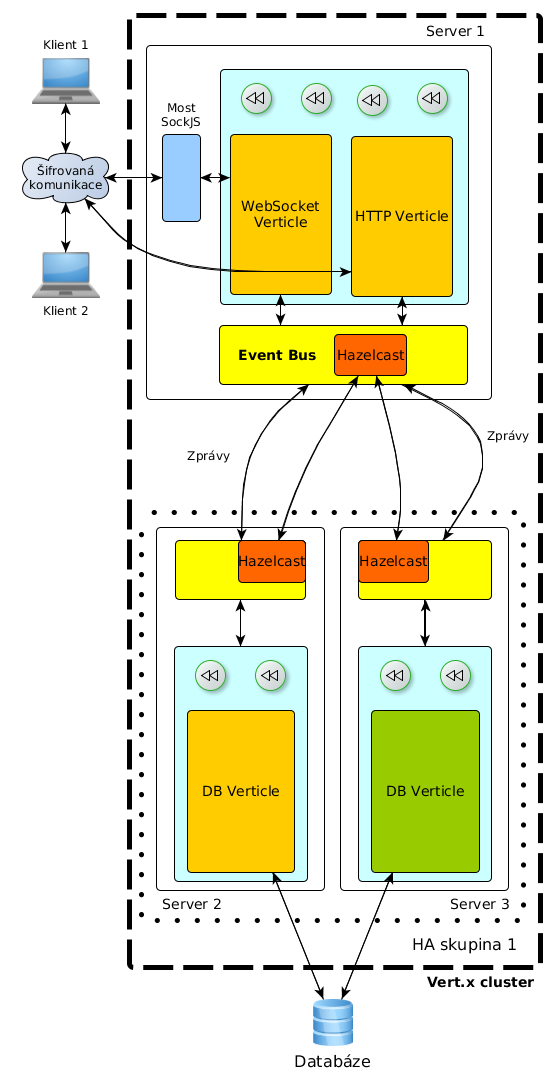
\includegraphics[scale=0.5]{obrazky/instance4_eventbus_geolocation}
\par\end{centering}
\caption{Clustering mezi třemi Vert.x instancemi \label{fig:instance4_eventbus_geolocation}}
\end{figure}

\subsection{Vysoká dostupnost}

Samostatnou kapitolou v oblasti clusteringu je HA\footnote{HA - High Availability} česky tedy vysoká dostupnost. Díky Hazelcastu ji lze řešit již na aplikační úrovni, a není potřeba  dalších služeb, které řeší vysokou dostupnost.

\subsubsection{Automatické zotavení z havárie}

Pokud je modul spuštěn s argumentem \emph{-ha} a dojde k pádu Vert.x instance. Modul bude automaticky nasazen na jiné instanci v clusteru. V takovém případě již není potřeba spouštět modul s parametrem \emph{-cluster}. Jak je vidět na obrázku \ref{fig:instance4_eventbus_geolocation} v případě pádu Serveru 2, tedy části aplikace, která komunikuje s databází dojde automaticky k novému nasazení této části do nové instance.

\subsubsection{Skupiny HA}

V případě spuštění modulů v režimu HA lze pak specifikovat logické skupiny. Díky tomu lze určit, kde se mají moduly v případě pádu nasadit. Z toho logicky vyplývá, že moduly se nasadí jen na instancích se stejnou HA skupinou.

\subsubsection{Kvorum}

Při spuštění Vert.x instance lze specifikovat kvorum\footnote{minimální počet serverů pro zajištění vysoké dostupnosti}. Pokud nebude splněno kvorum nebude instance nasazena v režimu HA. Kvorum lze pak snadno spočítat ze vzorce \emph{Q = 1 + N/2}, kde N je počet serverů. Pokud dojde při běhu aplikace k porušení kvora bude režim HA automaticky vysazen.

\section{Porovnání s Node.js}

V následující kapitole bude porovnána platforma Vert.x s již zmíněnou platformou Node.js. Výkonnostní test\cite{benchmarkTim} je převzat od samotného autora projektu a jsou v něm zahrnuty jazyky, které v té době platforma podporovala. V druhé části kapitoly \ref{sub:performence} je pak tabulka\ref{table:odezvy} srovnání odezev s vybranými webovými platformami z daty ze zdroje\cite{benchmark}.

\subsection{Výkon}\label{sub:performence}

Tato kapitola se zabývá výkonnostními testy jednotlivých platforem. V prvním testu je obsaženo více programovacích jazyků, ve kterých byla implementována stejná logika pod platformou Vert.x. Rychlost aplikace implementované v jiném jazyce než Javě je pak závislá na konkrétním adaptéru.

\subsubsection{Metody testování}

V obou testech je testovaná aplikace škálovaná na šest procesorových jader tedy byla spuštěna s parametrem \emph{-instances 6}, oproti tomu je spuštěna aplikace Node.js ve dvou variantách. Samostatná a šest procesů v jednom clusteru. V legendě grafů je to odlišeno příponou \emph{cl}.

\begin{enumerate}
\item{Triviální dotazování serveru a návrat statusu 200\footnote{HTTP status - OK}}
\item{Dotaz na statický soubor o velikosti 72 bytů}
\end{enumerate}

\subsubsection{Hardware}

V prvním testu od Tima Foxe je požit  AMD Phenom II X6, 8GB RAM a systém Ubuntu 11.04. Tento procesor se 6 jádry není úplně běžný proto je výklad doplněn o druhý test, který proběhl na Sandy Bridge Core i7-2600K, 8GB RAM a SSD disku a systému Ubuntu 12.04.

\subsubsection{Výsledky}

Jak lze vidět na obrázku \ref{fig:test1} a \ref{fig:test2} výsledky obou testů lze shrnout do jedné věty. Vert.x zvládá řádově o desítky tisíc více odpovědí než platforma Node.js a i v případě režimu clusteru.

\begin{figure}
\begin{centering}
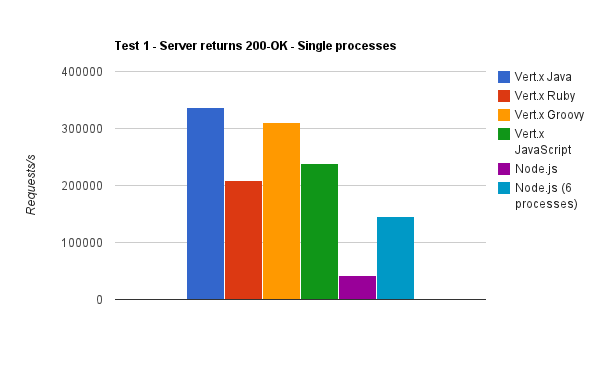
\includegraphics[scale=0.7]{obrazky/chart_1}
\par\end{centering}
\caption{Výsledky druhého testu \emph{Tim Fox} \label{fig:test1}}
\end{figure}

\begin{figure}
\begin{centering}
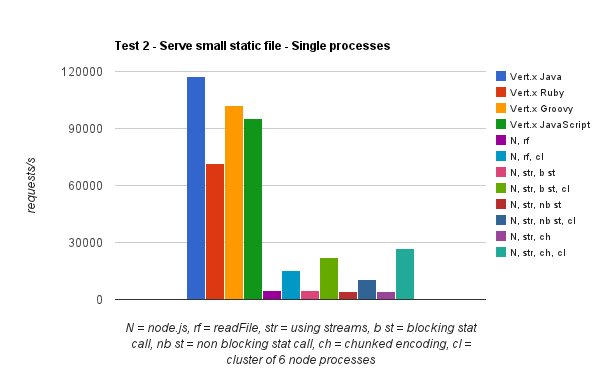
\includegraphics[scale=0.7]{obrazky/chart_3-5}
\par\end{centering}
\caption{Vert.x instance \emph{Výsledek druhého testu Tim Fox} \label{fig:test2}}
\end{figure}

\subsubsection{Srovnání s vybranými platformami}

Metoda srovnání s ostatními platformami je založená na podobném principu jako předchozí testy s tím rozdílem, že místo statického souboru vrací odpověď ve formátu JSON. Na straně serveru tedy musí dojít k JSON serializaci.

\begin{flushleft}
\begin{longtable}{|c|c|c|}
\hline
\textsf{\textbf{Platforma}} & \textsf{\textbf{Průměrná odezva}} & \textsf{\textbf{Maximální}}\tabularnewline
\hline
Vert.x & 1,2ms & 18,7ms\tabularnewline
\hline 
Netty & 1,3ms & 24,0ms\tabularnewline
\hline
Ruby on Rails & 1.8ms & 241.6\tabularnewline
\hline 
Node.js & 3.7ms & 12,5\tabularnewline
\hline 

\caption{Srovnání odezvy}
\label{table:odezvy}
\end{longtable}
\end{flushleft}

\subsection{Vlastnosti}

Následující tabulka ukazuje srovnání důležitých vlastností jednotlivých platforem, jejichž důležitost byla popsána v předchozích kapitolách.

\begin{flushleft}
\begin{longtable}{|c|c|c|}
\hline
\textsf{\textbf{Vlastnost}} & \textsf{\textbf{Node.js}} & \textsf{\textbf{Vert.x}}\tabularnewline
\hline
CLI & Ano & Ano\tabularnewline
\hline 
Cluster & Ano & Ano\tabularnewline
\hline
Moduly & Ano & Ano\tabularnewline
\hline 
HA & Ne & Ano\tabularnewline
\hline
MQ & Ne & Ano\tabularnewline
\hline 
Hybridní model vláken & Ne & Ano\tabularnewline
\hline 
In-memory data grid & Ne & Ano\tabularnewline
\hline 
Polygnot & Ne & Ano\tabularnewline
\hline
\caption{Srovnání vlastností s Node.js}
\end{longtable}
\par\end{flushleft}

\subsection{Závěr srovnání}

Výsledkem srovnání je tedy fakt, že pokud by se dnes někdo rozhodoval o výběru platformy pro novou real-time aplikaci měl by určitě zvolit platformu Vert.x, která poskytuje řádově větší výkon a počet vlastností, nehledě na fakt, že v případě Node.js lze psát aplikaci pouze v jazyce JavaScipt, který se může jevit jako naprosto nevhodný pro Enteprise aplikaci.